\begin{frame}{Semana 1 (06/02/2024) - T1}
        \textbf{Trabajo}

        $$W_{12}=\int_{1}^{2}\vec{\boldsymbol{F}}\boldsymbol{\cdot} d\vec{\boldsymbol{s}}.$$
\end{frame}

\begin{frame}{Semana 1 (06/02/2024) - T1P1}

La masa del niño es $m$, la longitud
de las cadenas es $R$, y se empuja con una fuerza $F$ hasta que las cadenas forman un
ángulo $\theta_0$ con la vertical. La fuerza $F$ es horizontal, variable, comienza en cero y aumenta en forma gradual apenas lo suficiente para que el niño y el columpio se muevan lentamente y permanezcan casi en equilibrio.

¿Qué trabajo total realizan todas las
fuerzas sobre el niño? ¿Qué trabajo realiza la tensión en las cadenas? ¿Qué trabajo efectúa la fuerza $F$? (Ignore el peso
de las cadenas y el asiento).

\begin{figure}[H]
    \centering
    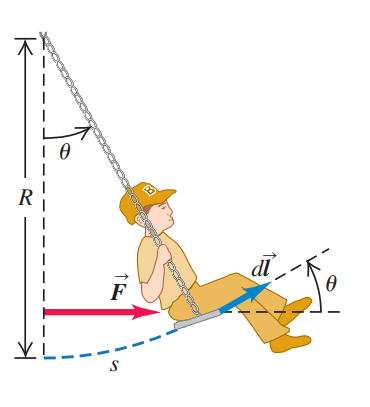
\includegraphics[width=0.3\textwidth]{figures/t1t1.png}
\end{figure}
    
\end{frame}

\begin{frame}{Semana 1 (06/02/2024) - T1}
    \textbf{Energía cinética}
    $$W_{12}=K_2-K_1=\frac{m}{2}\left(v_2^2-v_1^2\right).$$
    
    \textbf{Energía potencial}
    
    Si $W_{12}$ es independiente de la trayectoria:
    $$W_{12}=U_1-U_2,$$
    $$\vec{\boldsymbol{F}}=-\vec{\boldsymbol{\nabla}}U(\vec{\boldsymbol{r}}),$$
    $$\oint_1^2\vec{\boldsymbol{F}}\boldsymbol{\cdot} d\vec{\boldsymbol{s}}=0.$$
    
    \textbf{Conservación de la energía}
    $$K_1+U_1=K_2+U_2.$$
\end{frame}

\begin{frame}{Semana 1 (06/02/2024) - T1P2}

    \textbf{Atwood's Machine}

    \begin{figure}[H]
    \centering
    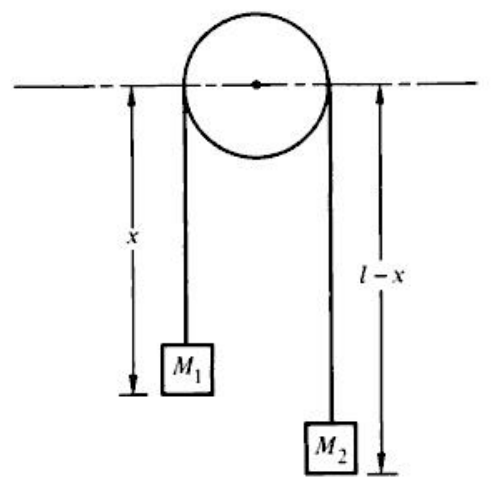
\includegraphics[width=0.5\textwidth]{figures/t1t2.png}
\end{figure}
    
\end{frame}